\documentclass{article}

\usepackage{amsmath}
\usepackage{amssymb}
\usepackage[left=1in, right=1in]{geometry}
\usepackage{graphicx}
\usepackage{subcaption}

\title{Project Accordian}
\author{Documentation for Software Version $1.0$}

\begin{document}
\maketitle

\section{Abstract}
The goal of this project is to come up with a new way of operating a hand-held computer (smartphone, netbook laptop, PDA, etc). At the moment, the technology is tranding towards greater reliance on touchscreen operation. This has many advantages, such as context-aware keyboard representation, efficient use of physical space. However, there are some drawbacks. Touch typing is impossible, accidental presses are a possibility, and it uses valuable screen space, all detrimental to productivity and not particularly conducive to good workflow. Physical keyboards (of the type that big fruity mobile-phone manufacturer is famous for --- not that one, the other fruity one) are a step in the right direction. Physical keys enable much faster typing, even touch typing, but still doesn't come as close to a streamlined workflow as is possible. There are only a limited number of keys, and as with most phone keyboards, only up to two fingers (thumbs) can operate the device at a time. Project Accordian is a new design to hopefully solve these issues and make smartphones a viable device for work, not just a communication device.

\begin{figure}[!h]
	\centering
	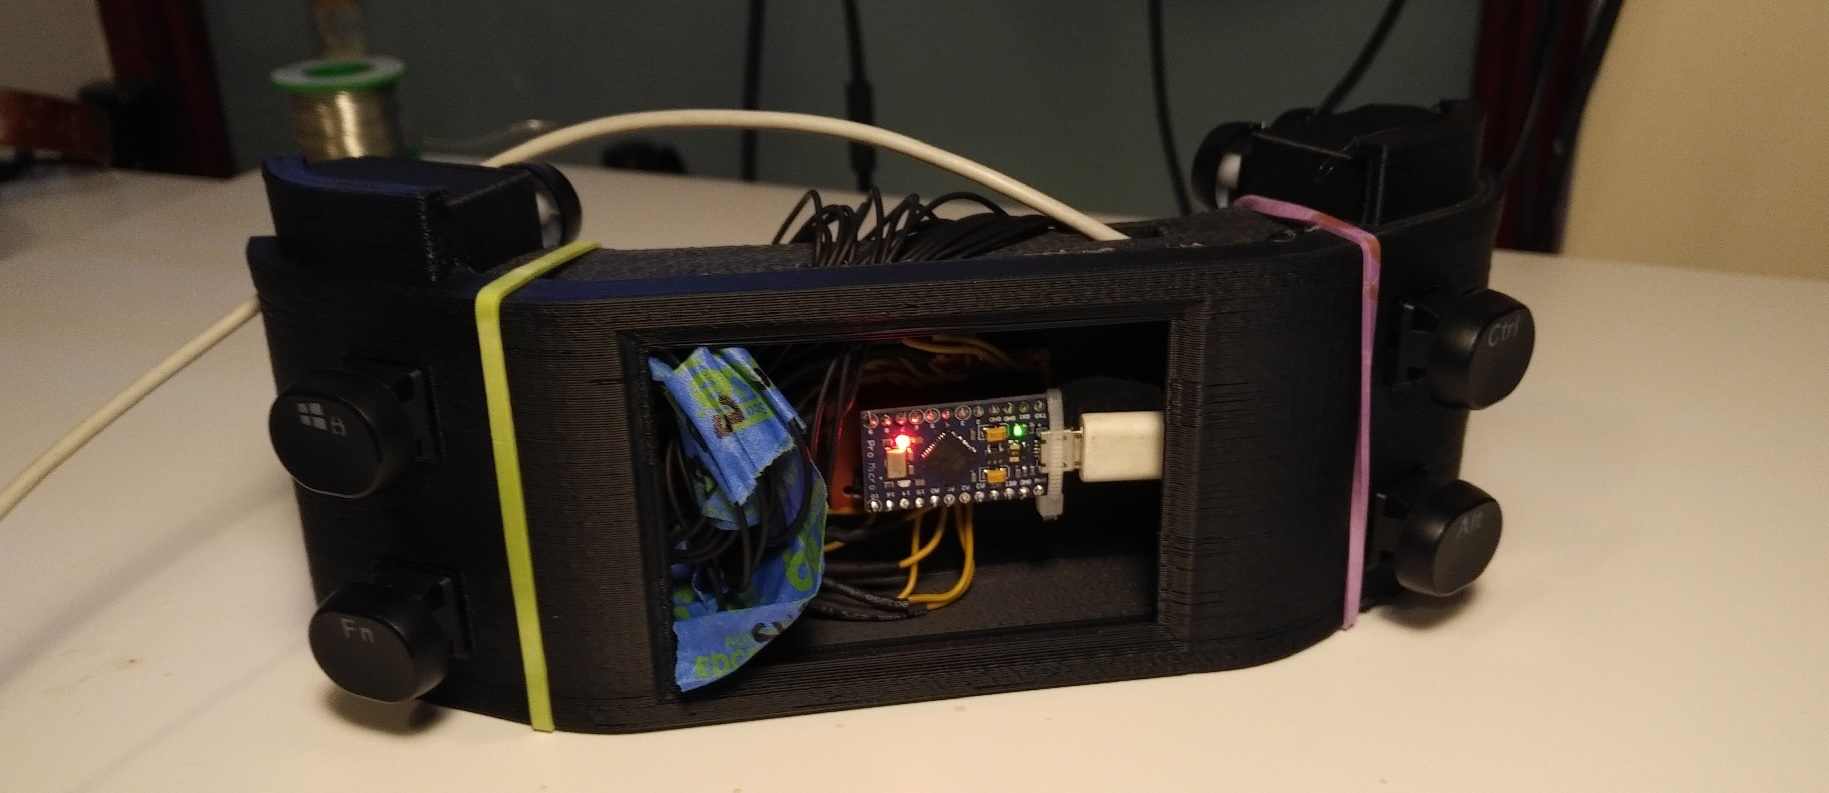
\includegraphics[width=.6\textwidth]{imgs/5_pro3.jpg}
	\caption{\label{proto2} Prototype v2 ``Swtch-PSP-ish''}
\end{figure}

\section{Specification}
Project Accordian should:
\begin{itemize}
	\item be faster to use than a standard phone keyboard
	\item have access to all $\sim$100 keys as on a standard windows-style keyboard
	\item be workable for portable devices (mobile phone, tablet) --- perhaps as some sort of case mod?
	\item be as open source as is possible.
\end{itemize}

Optionally:
\begin{itemize}
	\item be usable one-handed
	\item be modular (one device, many modes)
\end{itemize}

\section{Solution}
Keys will be split into different categories: numbers (0-9), letters (a-z), symbols (\&, ?, !, ", etc), modifiers (Ctrl, Shift, Win, Alt, Alt Gr), and misc (Up, Down, Return, Del, Esc, etc).

%Each category (excluding modifiers) will be accessible by selecting the category (left index finger, four buttons). Then, groups of 8 keys in the category can be selected (left middle, ring, and pinky, two buttons each). Finally, the desired key is typed using the right hand buttons (two per finger). This corresponds to ($4 \times 3 \times 2 \times 4 \times 2 = 192$)
Each category (excluding modifiers) will be split into groups of 8 keys, selectable using the four left hand keys. Then, the individual keys can be typed using the right hand set of keys. This gives a total set of ($2^4 \times 8 = 128$) key combinations.

\section{Key Map}

Selection is split into four groups of four sub-groups of similar keys: \textbf{Alphabet}, \textbf{Numerical}, \textbf{Symbols}, and \textbf{Misc}. To select each, press the main group selector with your ring and pinky fingers, then count in binary from 0-3 with your index and middle fingers (index is always LSB).

\subsection{Alphabet}
This group consists simply of four sets comprising the alphabet a-h, i-p, q-x, y-z. Selected number 1 (ring finger down only).
\begin{center}
	\begin{table}[!h]
		\begin{subtable}{0.45\textwidth}
			\centering
			\begin{tabular}{|c|c|c|c|c|}
				\hline
				\multicolumn{5}{|c|}{ALPHA1}\\ \hline
				  & I & M & R & P \\ \hline
				T & a & b & c & d \\ \hline
				M & e & f & g & h \\ \hline
			\end{tabular}
		\end{subtable}
		\begin{subtable}{0.45\textwidth}
			\centering
			\begin{tabular}{|c|c|c|c|c|}
				\hline
				\multicolumn{5}{|c|}{ALPHA2}\\ \hline
				& I & M & R & P \\ \hline
				T & i & j & k & l \\ \hline
				M & m & n & o & p \\ \hline
			\end{tabular}
		\end{subtable}
	\end{table}
\end{center}

\begin{center}
	\begin{table}[!h]
		\begin{subtable}{0.45\textwidth}
			\centering
			\begin{tabular}{|c|c|c|c|c|}
				\hline
				\multicolumn{5}{|c|}{ALPHA3}\\ \hline
				& I & M & R & P \\ \hline
				T & q & r & s & t \\ \hline
				M & u & v & w & x \\ \hline
			\end{tabular}
		\end{subtable}
		\begin{subtable}{0.45\textwidth}
			\centering
			\begin{tabular}{|c|c|c|c|c|}
				\hline
				\multicolumn{5}{|c|}{ALPHA4}\\ \hline
				& I & M & R & P \\ \hline
				T & y & z & - & - \\ \hline
				M & - & - & - & - \\ \hline
			\end{tabular}
		\end{subtable}
	\end{table}
\end{center}

\subsection{Numerical}
One and a bit sub-groups consisting of the numbers 0 to 9. Selected group 2 (pinky finger down only).

\begin{center}
	\begin{table}[!h]
		\begin{subtable}{0.45\textwidth}
			\centering
			\begin{tabular}{|c|c|c|c|c|}
				\hline
				\multicolumn{5}{|c|}{MATHS1}\\ \hline
				& I & M & R & P \\ \hline
				T & 0 & 1 & 2 & 3 \\ \hline
				M & 4 & 5 & 6 & 7 \\ \hline
			\end{tabular}
		\end{subtable}
		\begin{subtable}{0.45\textwidth}
			\centering
			\begin{tabular}{|c|c|c|c|c|}
				\hline
				\multicolumn{5}{|c|}{ALPHA2}\\ \hline
				& I & M & R & P \\ \hline
				T & 8 & 9 & - & - \\ \hline
				- & - & - & - & - \\ \hline
			\end{tabular}
		\end{subtable}
	\end{table}
\end{center}

\subsection{Symbols}
This group comprises every special character in no particular order. Selected number 3 (both ring and pinky fingers down).

\begin{center}
	\begin{table}[!h]
		\begin{subtable}{0.45\textwidth}
			\centering
			\begin{tabular}{|c|c|c|c|c|}
				\hline
				\multicolumn{5}{|c|}{SYMBS1}\\ \hline
				& I & M & R & P \\ \hline
				T & $+$ & $-$ & $*$ & $/$ \\ \hline
				M & \textasciicircum & $=$ & \_ & - \\ \hline
			\end{tabular}
		\end{subtable}
		\begin{subtable}{0.45\textwidth}
			\centering
			\begin{tabular}{|c|c|c|c|c|}
				\hline
				\multicolumn{5}{|c|}{SYMBS2}\\ \hline
				& I & M & R & P \\ \hline
				T & $($ & $)$ & \% & \$ \\ \hline
				M & $<$ & $>$ & ! & $\neg$ \\ \hline
			\end{tabular}
		\end{subtable}
	\end{table}
\end{center}

\begin{center}
	\begin{table}[!h]
		\begin{subtable}{0.45\textwidth}
			\centering
			\begin{tabular}{|c|c|c|c|c|}
				\hline
				\multicolumn{5}{|c|}{SYMBS3}\\ \hline
				& I & M & R & P \\ \hline
				T & , & . & " & ? \\ \hline
				M & : & ; & ' & \# \\ \hline
			\end{tabular}
		\end{subtable}
		\begin{subtable}{0.45\textwidth}
			\centering
			\begin{tabular}{|c|c|c|c|c|}
				\hline
				\multicolumn{5}{|c|}{SYMBS4}\\ \hline
				& I & M & R & P \\ \hline
				T & @ & \& & $[$ & $]$ \\ \hline
				M & $\{$ & $\}$ & \textasciitilde & \textbackslash \\ \hline
			\end{tabular}
		\end{subtable}
	\end{table}
\end{center}

\subsection{Misc}
Finally, we have the default group. This group consists of a number of special keys used for navigation, or for generally dealing with forms and so on. In this group are also the twelve function keys. Selected group 0 (neither ring nor pinky pressed).

\begin{center}
	\begin{table}[!h]
		\begin{subtable}{0.45\textwidth}
			\centering
			\begin{tabular}{|c|c|c|c|c|}
				\hline
				\multicolumn{5}{|c|}{NAVIG1}\\ \hline
				& I & M & R & P \\ \hline
				T & $\leftarrow$ & $\uparrow$ & $\downarrow$ & $\rightarrow$ \\ \hline
				M & Home & End & PgUp & PgDn \\ \hline
			\end{tabular}
		\end{subtable}
		\begin{subtable}{0.45\textwidth}
			\centering
			\begin{tabular}{|c|c|c|c|c|}
				\hline
				\multicolumn{5}{|c|}{NAVIG2}\\ \hline
				& I & M & R & P \\ \hline
				T & Tab & Ret & Bkspc & Del \\ \hline
				M & Space & Esc & - & - \\ \hline
			\end{tabular}
		\end{subtable}
	\end{table}
\end{center}

\begin{center}
	\begin{table}[!h]
		\begin{subtable}{0.45\textwidth}
			\centering
			\begin{tabular}{|c|c|c|c|c|}
				\hline
				\multicolumn{5}{|c|}{FUNCS1}\\ \hline
				& I & M & R & P \\ \hline
				T & F1 & F2 & F3 & F4 \\ \hline
				M & F5 & F6 & F7 & F8 \\ \hline
			\end{tabular}
		\end{subtable}
		\begin{subtable}{0.45\textwidth}
			\centering
			\begin{tabular}{|c|c|c|c|c|}
				\hline
				\multicolumn{5}{|c|}{FUNCS2}\\ \hline
				& I & M & R & P \\ \hline
				T & F9 & F10 & F11 & F12 \\ \hline
				M & - & - & - & - \\ \hline
			\end{tabular}
		\end{subtable}
	\end{table}
\end{center}

\section{Future work}
Something of a to-do list:

\begin{itemize}
	\item Redesign shell
	\item Add support for some kind of touchpad (via the two remaining analogue pins on the arduino?)
	\item Optimize positioning of keys --- maybe something more closely related to QWERTY as it is basically ingrained into my (and most other people's) head.
	
	This could be tricky as the three lines of (purely letters) on a QWERTY keyboard are 10, 9, and 7 letters long.
\end{itemize}

\newpage\appendix
\section{Appendix A: Overall Key Map Table}

Fingers are referred to here by a simply notation: L for left-hand, R for right-hand. 0-3 for index  to pinky. Right hand has $_M$ for mid-keys, and $_T$ for tip-keys. So right pinky, middle key, would be R3$_M$. Left Index is L0.

\begin{center}
	\begin{tabular}{|cccc|c|cccc|cccc|}
		\hline
		\multicolumn{4}{|c|}{\textbf{Group Selector}} & \textbf{Name} & \multicolumn{4}{|c|}{\textbf{Tip Keys}} & \multicolumn{4}{|c|}{\textbf{Mid Keys}} \\ \hline
		L3 & L2 & L1 & L0 &  & R0$_M$ & R1$_M$ & R2$_M$ & R3$_M$ & R0$_T$ & R1$_T$ & R2$_T$ & R3$_T$ \\ \hline
		\multicolumn{13}{|c|}{\textbf{00xx --- Navigation group}}\\ \hline
		0 & 0 & 0 & 0 & NAVIG1 & Left & Up & Down & Right & Home & End & PgUp & PgDn \\ \hline
		0 & 0 & 0 & 1 & NAVIG2 & Tab & Return & Bkspc & Del & Space & Esc & -- & -- \\ \hline
		0 & 0 & 1 & 0 & FUNCS1 & F1 & F2 & F3 & F4 & F5 & F6 & F7 & F8 \\ \hline
		0 & 0 & 1 & 1 & FUNCS2 & F9 & F10 & F11 & F12 & -- & -- & -- & -- \\ \hline
		\multicolumn{13}{|c|}{\textbf{01xx --- Alphabet group}}\\ \hline
		0 & 1 & 0 & 0 & ALPHA1 & a & b & c & d & e & f & g & h \\ \hline
		0 & 1 & 0 & 1 & ALPHA2 & i & j & k & l & m & n & o & p \\ \hline
		0 & 1 & 1 & 0 & ALPHA3 & q & r & s & t & u & v & w & x \\ \hline
		0 & 1 & 1 & 1 & ALPHA4 & y & z & -- & -- & -- & -- & -- & -- \\ \hline
		\multicolumn{13}{|c|}{\textbf{10xx --- Maths group}}\\ \hline
		1 & 0 & 0 & 0 & MATHS1 & 0 & 1 & 2 & 3 & 4 & 5 & 6 & 7 \\ \hline
		1 & 0 & 0 & 1 & MATHS2 & 8 & 9 & -- & -- & -- & -- & -- & -- \\ \hline
		1 & 0 & 1 & 0 & --     & -- & -- & -- & -- & -- & -- & -- & -- \\ \hline
		1 & 0 & 1 & 1 & --     & -- & -- & -- & -- & -- & -- & -- & -- \\ \hline
		\multicolumn{13}{|c|}{\textbf{11xx --- Symbols group}}\\ \hline
		1 & 1 & 0 & 0 & SYMBS1 & $+$ & $-$ & $*$ & $/$ & \textasciicircum & $=$ & \_ & -- \\ \hline
		1 & 1 & 0 & 1 & SYBMS2 & $($ & $)$ & \% & \$ & $<$ & $>$ & ! & $\neg$ \\ \hline
		1 & 1 & 1 & 0 & SYMBS3 & , & . & ? & " & : & ; & ' & \# \\ \hline
		1 & 1 & 1 & 1 & SYMBS4 & @ & \& & $[$ & $]$ & $\{$ & $\}$ & \textasciitilde & \textbackslash \\ \hline
		
	\end{tabular}
\end{center}

Then, each thumbs has the four modifier keys available: Ctrl, Shift, Alt, and Super, as well as Esc (left) and Space (right).
\end{document}
